% MASooda: BMS-in-the-loop traffic management for urban drone fleets
% Target: IEEE Access (compiles with the standard IEEEtran class in journal mode;
% port to the IEEE Access template before submission).
\documentclass[journal]{IEEEtran}

\usepackage{cite}
\usepackage{amsmath,amssymb}
\usepackage{graphicx}
\usepackage{booktabs}
\usepackage{multirow}
\usepackage{algorithm}
\usepackage{algorithmic}
\usepackage{tikz}
\usetikzlibrary{positioning,arrows.meta,fit,calc}
\usepackage{xcolor}
\usepackage{url}

\newtheorem{proposition}{Proposition}
\newcommand{\socH}{\widehat{\mathrm{SoC}}}
\newcommand{\Ebms}{E^{\mathrm{BMS}}}
\newcommand{\Eneed}{E^{\mathrm{need}}}

\begin{document}

\title{BMS-in-the-Loop Traffic Management for Urban Drone Fleets: Chance-Constrained Energy Reserves, Pad Arbitration, and Energy-Weighted ADMM Deconfliction}

\author{R~Lalith~Vishnu,
        Sampadram,
        Mohammed~Abdur~Rehman,
        Bhuvan,
        Tanmay~Banjari,
        and~Dhadheechi%
\thanks{The authors are with the Indian Institute of Technology Hyderabad, Kandi, Sangareddy, Telangana 502284, India (e-mail: [to be completed]).}%
\thanks{Code and simulator: \url{https://github.com/rlv-iith/MASooda}.}}

\markboth{Manuscript draft}{Lalith Vishnu \MakeLowercase{\textit{et al.}}: BMS-in-the-Loop Traffic Management for Urban Drone Fleets}

\maketitle

\begin{abstract}
%%ABSTRACT%%
\end{abstract}

\begin{IEEEkeywords}
Unmanned aircraft system traffic management (UTM), battery management system, state-of-charge estimation, chance constraints, ADMM, multi-agent systems.
\end{IEEEkeywords}

%======================================================================
\section{Introduction}
\IEEEPARstart{L}{ow}-altitude delivery and emergency drones are battery-electric, and their endurance is the binding constraint on almost every operational decision: whether to take off, whether to continue, where to land, and how much a conflict manoeuvre may cost. Policy documents already anticipate this. India's National UTM Policy Framework lists real-time health and status monitoring and contingency management among UTM services~\cite{indiaUTM2021}; NASA's In-time Aviation Safety Management System concept names vehicle-health monitors and battery prognostics as services that can trigger automatic mitigation~\cite{ellis2021iasms}; the FAA UTM concept of operations, by contrast, leaves endurance to the operator~\cite{faa2020conops}.

The traffic-management algorithms themselves are, however, largely energy-agnostic. Tactical deconfliction priorities are derived from the operation class and manoeuvrability~\cite{jover2022priority}, separation assurance between heterogeneous fleets models equipage and sensing rather than energy~\cite{sharifi2026separation}, and distributed trajectory optimisation handles collision and kinematic constraints only~\cite{ni2022admm}. When energy enters, it does so before the flight~\cite{liu2017energy}, at the arrival schedule~\cite{kleinbekman2018evtol}, or as a cost that is measured after conflicts have been resolved~\cite{zongo2026overhead}. Conversely, battery prognostics and health management (PHM) for electric aircraft is mature~\cite{saha2011bhm,bole2014online,kulkarni2018remaining,hogge2024octocopter,kulkarni2024thermal}, but its decisions---abort, replan, re-route to a landing site---are taken by a single vehicle that does not know the surrounding traffic or the occupancy of the landing pads~\cite{taye2025safe,quinones2020decision,montazeri2024health,baculi2019onboard}.

This paper closes the loop between the battery management system (BMS) of each drone and the traffic manager of the fleet. The setting is MASooda, a hierarchical multi-agent traffic-management simulator built on road-aligned corridors traced from the campus of IIT Hyderabad. Each drone carries an equivalent-circuit battery model with per-cell spread and a lumped thermal model, and its BMS estimates the state of charge, the polarisation voltage and the capacity with an extended Kalman filter (EKF) from noisy, biased sensors. Every energy decision, onboard or at the traffic controller, uses a one-sided chance-constrained energy bound and a weakest-cell voltage check rather than the true state. The traffic controller then uses the same BMS state in three places: it gives drones in a critical health state right of way, it arbitrates landing pads by remaining endurance, and it raises a drone's weight in the ADMM conflict resolver continuously as its energy margin shrinks.

The contributions are:
\begin{enumerate}
\item An open, reproducible hierarchical traffic-management simulator for urban drone fleets that combines local car-following and boids-style coordination, consensus-ADMM conflict resolution, a priority-aware drone traffic controller (DTC) with a reserved emergency layer, trusted-range and W-MSR filtering of position reports, and layer-aware signal temporal logic (STL) monitoring (Section~\ref{sec:system}).
\item A BMS-in-the-loop decision layer: a 1-RC Thevenin pack model with weakest-cell usable energy, an EKF on $(\mathrm{SoC}, V_{RC}, 1/Q)$, and a feasibility test that combines a chance-constrained energy bound with a voltage-sag check (Sections~\ref{sec:battery}--\ref{sec:estimation}).
\item Two fleet-level uses of that state: endurance-ordered landing-pad arbitration with hold-short of non-urgent arrivals, and a continuous, bounded ADMM weight derived from the energy margin (Section~\ref{sec:health}).
\item A paired-seed evaluation on the campus map that separates the contribution of the traffic manager from that of the state estimate, together with architecture, resilience, scaling and link-outage experiments (Section~\ref{sec:results}).
\end{enumerate}

Section~\ref{sec:related} reviews related work, Sections~\ref{sec:system}--\ref{sec:health} describe the method, Section~\ref{sec:impl} the implementation, Section~\ref{sec:results} the experiments, and Section~\ref{sec:discussion} the limitations.

%======================================================================
\section{Related Work}\label{sec:related}

\subsection{Priority-Aware and Distributed Deconfliction}
Jover \textit{et al.}~\cite{jover2022priority} extend the PCAN tactical algorithm for U-space with a priority derived from the operation class and manoeuvrability; lower-priority drones absorb most of the deviation (up to 8\% more distance and 17\% more flight time) with no conflicts among 100 UAVs. Learning-based separation assurance between heterogeneous fleets~\cite{sharifi2026separation} and edge-AI conflict management~\cite{agnihotri2025swarm} optimise separation, latency and accuracy, but do not model the energy or health of the vehicles. ADMM has been applied to robust multi-robot trajectory optimisation with collision and kinematic constraints~\cite{ni2022admm}; MASooda uses consensus ADMM~\cite{boyd2011admm} for short-horizon velocity negotiation in the same spirit. None of these works lets the energy state decide who manoeuvres.

\subsection{Energy in Traffic Management}
Liu and Sengupta plan flights to minimise energy~\cite{liu2017energy}. Kleinbekman \textit{et al.}~\cite{kleinbekman2018evtol} include each eVTOL's state of charge in a mixed-integer arrival-sequencing model, so that the latest feasible arrival time follows from the remaining charge. KrisshnaKumar \textit{et al.}~\cite{krisshnakumar2023vertiport} include battery level in the state and reward of a learned vertiport take-off and landing scheduler. Zongo and Wei~\cite{zongo2026overhead} quantify the energy overhead of conflict resolution in high-density airspace: the median is below 1.5\%, but the tail reaches 44\%, and the battery state does not feed back into how conflicts are resolved. SkyGrid~\cite{khoshdel2024skygrid} balances energy and throughput at aerial intersections.

\subsection{Battery Health Management for a Single Vehicle}
Battery health management for electric UAVs predicts end of discharge with particle filters~\cite{saha2011bhm} or unscented Kalman filters~\cite{bole2014online}, provides flight-tested remaining-flying-time alarms~\cite{kulkarni2018remaining,hogge2024octocopter}, and couples prognostics with thermal models~\cite{kulkarni2024thermal}. Decision layers built on these estimates are single-vehicle: real-time mission feasibility checks that re-route to the nearest landing site~\cite{taye2025safe}, risk-based trajectory selection~\cite{quinones2020decision}, health-aware mission and altitude planning with reinforcement learning~\cite{montazeri2024health}, and onboard contingency managers that move from nominal flight to ``land now''~\cite{baculi2019onboard}. Extended Kalman filtering of equivalent-circuit models is the established BMS technique~\cite{plett2004ekf,plett2015bms}.

\subsection{Standards and Regulation}
ASTM F3548-21 defines operational-intent states, including non-conforming and contingent, for UTM service-supplier interoperability~\cite{astmF3548}. India's drone rules limit the green zone to 400~ft above ground level and to 200~ft in the 8--12~km band around an airport~\cite{pib2021drone}; MASooda's layer stack is placed inside the 400~ft ceiling.

\subsection{Positioning}
Table~\ref{tab:related} summarises the comparison. Prior work either manages traffic without the live battery state, or uses the battery state for one vehicle without the traffic. The present work uses an estimated, uncertainty-aware BMS state inside tactical fleet decisions---priority, pad allocation and ADMM weights---and measures the effect of each element separately.

\begin{table*}[t]
\centering
\caption{Battery state in related traffic-management and health-management work}
\label{tab:related}
\footnotesize
\begin{tabular}{@{}p{0.17\textwidth}p{0.13\textwidth}p{0.22\textwidth}p{0.22\textwidth}p{0.14\textwidth}@{}}
\toprule
Work & Scope & Battery information used & Decision it affects & Tactical deconfliction \\
\midrule
Jover \textit{et al.}~\cite{jover2022priority} & fleet (U-space) & none & priority by operation class & yes \\
Zongo and Wei~\cite{zongo2026overhead} & fleet (en route) & energy overhead, measured & none (reserve sizing) & yes (MVP) \\
Kleinbekman \textit{et al.}~\cite{kleinbekman2018evtol} & arrivals at a vertiport & SoC constraint & arrival schedule & no \\
KrisshnaKumar \textit{et al.}~\cite{krisshnakumar2023vertiport} & vertiport & battery level & take-off/landing scheduling & no \\
Taye \textit{et al.}~\cite{taye2025safe} & single vehicle & predicted voltage & reroute to landing site & no \\
Quinones-Grueiro \textit{et al.}~\cite{quinones2020decision} & single vehicle & SoC, remaining life & trajectory selection & no \\
Montazeri \textit{et al.}~\cite{montazeri2024health} & single vehicle & forecast voltage curve & mission order, altitude & no \\
\textbf{This work} & \textbf{fleet (campus)} & \textbf{EKF SoC, $V_{RC}$, capacity; cell voltages} & \textbf{priority, pad, ADMM weight, divert} & \textbf{yes (ADMM)} \\
\bottomrule
\end{tabular}
\end{table*}

%======================================================================
\section{System Overview}\label{sec:system}

\subsection{Airspace}
Corridors follow the road network: 28 road polylines traced from the IIT Hyderabad campus map form a graph of 105 junctions with 13 vertiports (one hospital, three depots, nine hubs), enclosed by a geofence (Fig.~\ref{fig:map}). Each corridor is a tube of width 20~m; inside it, each direction keeps to its own lane. Seven altitude layers are stacked 15~m apart starting at 30~m above ground ($L_0$--$L_6$ = 30--120~m); following the semicircular rule, eastbound traffic uses even and westbound traffic odd layers, and $L_6$ is reserved for medical emergencies. The campus is partitioned into six sectors; each (sector, layer) cell has a nominal capacity of 15 drones. Three mission types share the airspace: emergency (priority 0), passenger eVTOL (priority 1) and parcel delivery (priority 2).

\begin{figure}[t]
\centering
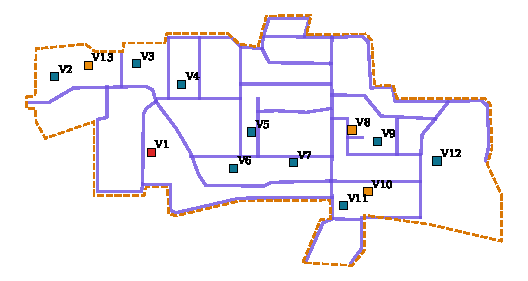
\includegraphics[width=\columnwidth]{fig_map.pdf}
\caption{Road-aligned corridor graph of the IIT Hyderabad campus used in all experiments (traced from the campus map). Squares mark vertiports; the dashed line is the geofence.}
\label{fig:map}
\end{figure}

\subsection{Hierarchical Architecture}
Fig.~\ref{fig:arch} shows the two tiers. Each drone follows its corridor route with a reference speed that brakes to stop at the pad, a car-following law $v \le (g - d_0)/h$ with $d_0 = 12$~m and $h = 1$~s, boids-style separation, alignment and along-road cohesion~\cite{reynolds1987flocks}, and closest-point-of-approach avoidance. Drones within 40~m exchange position reports over vehicle-to-vehicle (V2V) links. Before each tick, conflicting groups (pairs closer than the ADMM detection radius of 20~m on the same layer) negotiate their next positions with consensus ADMM (Section~\ref{sec:admm}).

The DTC runs every 2~s. It counts the load of every (sector, layer) cell, keeps emergencies on the reserved layer, moves drones out of over-capacity cells subject to a safety gate that defers a layer change if the target layer is occupied nearby, and settles layer requests from drones that are stuck behind slower traffic; drones also negotiate layers among themselves over V2V with consensus-based congestion prices. Operators can hold, reroute, ground, return to base, quarantine, impose speed limits, ground stops and temporary flight restrictions. If the DTC link fails, drones continue on their last directive and commands are queued.

Position reports pass a trusted-range check: a report that disagrees with the sensed range by more than 3~m is moved along its bearing to the sensed range, and W-MSR~\cite{leblanc2013resilient} with $f = 1$ fuses neighbour reports. Safety is monitored with the STL formula $\varphi = \mathbf{G}(d_{ij}(t) \ge d_{\min})$, $d_{\min} = 8$~m, through its robustness $\rho(t) = \min_{i \ne j} d_{ij}(t) - d_{\min}$~\cite{donze2010robust,fainekos2009robustness}, where $d_{ij}$ is the layer-aware distance $\|(\Delta x, \Delta y, \Delta L \cdot 15\,\mathrm{m})\|$.

\begin{figure}[t]
\centering
\resizebox{\columnwidth}{!}{%
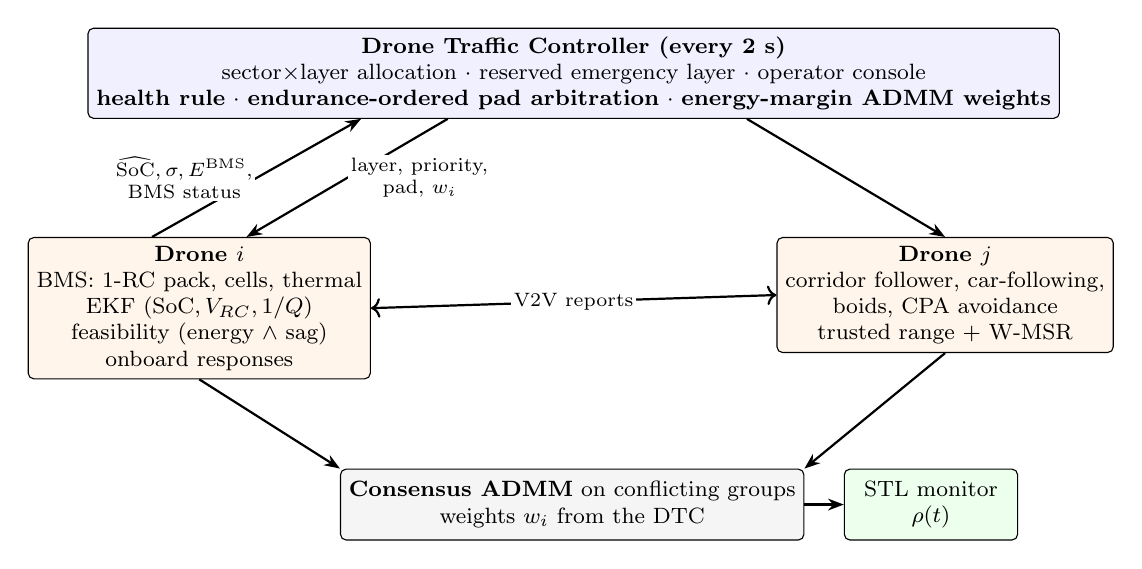
\begin{tikzpicture}[
  box/.style={draw, rounded corners=2pt, align=center, font=\footnotesize, minimum height=0.9cm, inner sep=3pt},
  dtc/.style={box, fill=blue!6},
  drone/.style={box, fill=orange!8},
  mon/.style={box, fill=green!7},
  arr/.style={-{Stealth[length=2mm]}, thick},
  lab/.style={font=\scriptsize, align=center, fill=white, inner sep=1pt}]
\node[dtc, minimum width=8.2cm] (dtc) {\textbf{Drone Traffic Controller (every 2 s)}\\
sector$\times$layer allocation $\cdot$ reserved emergency layer $\cdot$ operator console\\
\textbf{health rule} $\cdot$ \textbf{endurance-ordered pad arbitration} $\cdot$ \textbf{energy-margin ADMM weights}};
\node[drone, below left=1.5cm and -3.6cm of dtc, minimum width=3.9cm] (d1) {\textbf{Drone $i$}\\
BMS: 1-RC pack, cells, thermal\\ EKF $(\mathrm{SoC},V_{RC},1/Q)$\\ feasibility (energy $\wedge$ sag)\\ onboard responses};
\node[drone, below right=1.5cm and -3.6cm of dtc, minimum width=3.9cm] (d2) {\textbf{Drone $j$}\\
corridor follower, car-following,\\ boids, CPA avoidance\\ trusted range + W-MSR};
\node[box, below=1.3cm of $(d1.south)!0.5!(d2.south)$, minimum width=5.4cm, fill=gray!8] (admm) {\textbf{Consensus ADMM} on conflicting groups\\ weights $w_i$ from the DTC};
\node[mon, right=0.5cm of admm, minimum width=2.2cm] (stl) {STL monitor\\ $\rho(t)$};
\draw[arr] ($(d1.north)+(-0.6,0)$) -- node[lab, left]{$\socH,\sigma,\Ebms$,\\ BMS status} ($(dtc.south)+(-2.7,0)$);
\draw[arr] ($(dtc.south)+(-1.6,0)$) -- node[lab, right]{layer, priority,\\ pad, $w_i$} ($(d1.north)+(0.6,0)$);
\draw[arr] ($(dtc.south)+(2.2,0)$) -- ($(d2.north)+(0,0)$);
\draw[arr, <->] (d1.east) -- node[lab]{V2V reports} (d2.west);
\draw[arr] (d1.south) -- (admm.north west);
\draw[arr] (d2.south) -- (admm.north east);
\draw[arr] (admm.east) -- (stl.west);
\end{tikzpicture}}
\caption{MASooda architecture. Bold items are the BMS-in-the-loop elements introduced in this paper: the BMS estimate and feasibility test onboard, and their three uses by the DTC.}
\label{fig:arch}
\end{figure}

\subsection{Consensus ADMM Conflict Resolution}\label{sec:admm}
For a conflicting group $\mathcal{G}$ with positions $p_i$ and intended positions $t_i = p_i + v_i\,\Delta t$, the resolver solves
\begin{align}
\min_{\{x_i\}} \; & \sum_{i \in \mathcal{G}} \tfrac{w_i}{2}\,\|x_i - t_i\|^2 \label{eq:admm}\\
\text{s.t.}\; & n_{ij}^{\top}(x_i - x_j) \ge d_s \quad \forall (i,j) \in \mathcal{P}, \nonumber\\
& \|x_i - p_i\| \le v_{\max}\Delta t \quad \forall i \in \mathcal{G}, \nonumber
\end{align}
where $n_{ij}$ is the unit vector from $p_j$ to $p_i$ (a convexification of the separation constraint), $d_s = 1.01\,d_{\min}$, $\mathcal{P}$ contains the pairs on the same layer that can reach each other within one tick, $v_{\max} = 15$~m/s and $\Delta t = 0.1$~s. Each agent keeps one copy of its variable per constraint; the $x$-update is closed form,
\begin{equation}
x_i = \frac{w_i t_i + \rho \sum_{k}(z_{ik} - u_{ik})}{w_i + \rho K_i},
\label{eq:xupdate}
\end{equation}
with $K_i$ the number of constraints that involve $i$, followed by a projection of each copy onto its constraint set and a scaled dual update~\cite{boyd2011admm}. The parameters are $\rho = 1$, absolute and relative tolerances $10^{-3}$ and $10^{-4}$, and at most 50 iterations; a group that does not converge keeps its intended velocities and is counted as a fallback. In the baseline, $w_i$ is the class weight $w^{c} = 10, 3, 1$ for priorities 0, 1, 2.

%======================================================================
\section{Vehicle Energy and Battery Model}\label{sec:battery}

\subsection{Power}
With thrust $T = mg$, hover-induced velocity $v_h = \sqrt{T/(2\rho_a A)}$ and airspeed $v = \|v_g - v_w\|$ (ground velocity minus wind), the mechanical and electrical power follow momentum theory with parasitic drag~\cite{leishman2006principles}:
\begin{align}
v_i &= \sqrt{-v^2/2 + \sqrt{v^4/4 + v_h^4}},\\
P_{\mathrm{mech}} &= T v_i / \mathrm{FM} + \tfrac{1}{2}\rho_a C_D A_f\, v^3 \;(+\, T v_{\mathrm{climb}} \text{ in a climb}),\\
P_{\mathrm{el}} &= P_{\mathrm{mech}}/(\eta\, h_m) + P_{\mathrm{av}},
\end{align}
where FM is the figure of merit, $\eta$ the propulsive efficiency, $h_m \in (0,1]$ the motor health and $P_{\mathrm{av}}$ the avionics load. Air density $\rho_a$ follows the standard atmosphere at the site elevation (542~m) and the ambient temperature; at 35~$^\circ$C it is 1.074~kg/m$^3$, which raises hover power by 3.4\% relative to 15~$^\circ$C. Table~\ref{tab:vehicles} lists the parameters of the three vehicle types.

\begin{table}[t]
\centering
\caption{Vehicle and pack parameters}
\label{tab:vehicles}
\footnotesize
\setlength{\tabcolsep}{3pt}
\begin{tabular}{@{}lrrr@{}}
\toprule
 & Delivery & Emergency & eVTOL \\
\midrule
Mass + payload (kg) & 6 + 2 & 10 + 3 & 450 + 100 \\
Rotors $\times$ diameter (m) & 4 $\times$ 0.38 & 6 $\times$ 0.55 & 16 $\times$ 1.5 \\
FM / $\eta$ & 0.65 / 0.80 & 0.65 / 0.80 & 0.70 / 0.85 \\
$C_D A_f$ (m$^2$) & 0.08 & 0.12 & 1.2 \\
Avionics (W) & 25 & 40 & 500 \\
Cells in series / $V_{\mathrm{nom}}$ (V) & 6 / 22.2 & 12 / 44.4 & 108 / 400 \\
Capacity (Wh) & 500 & 800 & 25\,000 \\
$R_0$ ($\Omega$) / $C_{\max}$ & 0.02 / 5 & 0.04 / 5 & 0.05 / 5 \\
Pack heat capacity (J/K) & 2500 & 4000 & 139\,000 \\
\bottomrule
\end{tabular}
\end{table}

\subsection{Equivalent Circuit and Cells}
The pack is a 1-RC Thevenin circuit~\cite{plett2015bms}. The $n_s$ series cells share one current but have seeded SoC offsets $\delta_k \sim \mathcal{N}(0, 0.4\%)$ and resistance factors $\varepsilon_k \sim \mathcal{N}(0, 3\%)$. Because the cell open-circuit-voltage (OCV) curve is piecewise linear, the pack OCV is $\mathrm{OCV} = n_s\, \mathrm{OCV}_c(\mathrm{SoC} + \bar\delta)$. With $R_0$ scaled for ageing and cold, $R_1 = 0.5 R_0$ and $\tau = R_1 C_1 = 20$~s,
\begin{align}
I &= \frac{E - \sqrt{E^2 - 4 R_0 P_{\mathrm{el}}}}{2R_0},\qquad E = \mathrm{OCV} - V_{RC},\\
V &= \mathrm{OCV} - V_{RC} - I R_0,\\
V_{RC}^{+} &= V_{RC}\,e^{-\Delta t/\tau} + R_1 (1 - e^{-\Delta t/\tau}) I,\\
\mathrm{SoC}^{+} &= \mathrm{SoC} - (I + I_f)\,\Delta t / (3600\, Q),
\end{align}
where $Q = Q_{\mathrm{nom}}\,\mathrm{SoH}$ and $I_f$ is an internal fault current (below). If $E^2 < 4R_0P_{\mathrm{el}}$, the requested power cannot be delivered. The energy drawn from the cells per tick, $\mathrm{OCV}\, I\, \Delta t$, equals the delivered energy plus the heat $I^2 R_0 + I V_{RC}$; the test suite checks this balance to $10^{-9}$.

\textbf{Weakest-cell usable energy.} Series cells give up the same charge, so the pack stops when its weakest cell reaches $\mathrm{SoC}_{\min} = 5\%$. With $s_k = \mathrm{SoC} + \delta_k$ and span $\Delta = \min_k s_k - \mathrm{SoC}_{\min}$,
\begin{equation}
E^{\mathrm{use}}(\mathrm{SoC}, Q) = Q \sum_{k=1}^{n_s} \int_{s_k - \Delta}^{s_k} \mathrm{OCV}_c(s)\, ds .
\label{eq:usable}
\end{equation}
For identical cells this reduces to the usual $Q\, n_s \int_{\mathrm{SoC}_{\min}}^{\mathrm{SoC}} \mathrm{OCV}_c$; after a cell failure the whole string loses the failed cell's missing span.

\subsection{Temperatures, BMS States and Faults}
Pack and motor temperatures follow first-order lumped models~\cite{bernardi1985energy}, $C_p \dot T_p = I^2 R_0 + I V_{RC} + q_f - (h_0 + h_1\sqrt{v})(T_p - T_{\mathrm{amb}})$ and $C_m \dot T_m = (1 - \eta h_m)P_{\mathrm{el}}^{\mathrm{prop}} - (h_{m0} + h_{m1}\sqrt{v})(T_m - T_{\mathrm{amb}})$, so a hovering drone cools worse than a cruising one. Every 0.5~s the BMS computes the cell voltages $V_k = \mathrm{OCV}_c(s_k) - I R_c (1 + \varepsilon_k)$, the imbalance $\max_k V_k - \min_k V_k$ and five categories (charge, pack temperature, motor temperature, imbalance, current), each with WARNING, CRITICAL and FAULT thresholds and hysteresis (Table~\ref{tab:bms}). The drone's status is the worst category. Five faults can be scheduled: capacity loss ($Q \leftarrow 0.7Q$), cell failure (one cell $-15\%$ SoC and $3\times$ resistance), overheating (an internal dissipation $q_f = 0.6\,P_{\mathrm{hover}}$ that also drains charge as $I_f = q_f/\mathrm{OCV}$), motor degradation ($h_m = 0.8$) and GNSS degradation (a sensor fault).

\begin{table}[t]
\centering
\caption{BMS thresholds (hysteresis: 2\% SoC, 3~$^\circ$C, 10~mV)}
\label{tab:bms}
\footnotesize
\setlength{\tabcolsep}{3pt}
\begin{tabular}{@{}llll@{}}
\toprule
Category & WARNING & CRITICAL & FAULT \\
\midrule
SoC (estimated) & $<30\%$ & $<15\%$ & any cell $<3.0$~V \\
Pack temperature & $>55$~$^\circ$C & $>65$~$^\circ$C & $>75$~$^\circ$C \\
Motor temperature & $>90$~$^\circ$C & $>110$~$^\circ$C & --- \\
Cell imbalance & $>50$~mV & $>100$~mV & --- \\
Current & $>0.8\,I_{\max}$ & $>I_{\max}$ & infeasible \\
Sensor & --- & --- & injected fault \\
\bottomrule
\end{tabular}
\end{table}

%======================================================================
\section{BMS State Estimation and Chance-Constrained Feasibility}\label{sec:estimation}

\subsection{Extended Kalman Filter}
The BMS does not observe the true state. It measures the pack current with a seeded gain error ($\sigma = 0.5\%$) plus noise of $0.2$~A and $1\%$ of the reading, and the pack voltage with noise $5\sqrt{n_s}$~mV. An internal fault current is not seen by the current sensor. The estimator state is $x = (\mathrm{SoC}, V_{RC}, q)$ with $q = 1/Q$, so that a capacity change is learnt rather than known. With measured current $\tilde I$,
\begin{align}
\socH^{-} &= \socH - \tilde I\,\Delta t\, \hat q / 3600, \\
\hat V_{RC}^{-} &= \hat V_{RC}\, e^{-\Delta t/\tau} + R_1 (1 - e^{-\Delta t/\tau}) \tilde I,\\
\hat V &= n_s\, \mathrm{OCV}_c(\socH^{-} + \bar\delta) - \hat V_{RC}^{-} - R_0 \tilde I,
\end{align}
and the measurement Jacobian is $H = [\,n_s\, \mathrm{OCV}_c'(\socH^{-} + \bar\delta),\; -1,\; 0\,]$. The cell offsets $\bar\delta$ and $R_0$ are assumed to be identified online from the cell voltages. Process noise is $10^{-6}$~s$^{-1}$ on SoC, $10^{-4}$~V$^2$/s on $V_{RC}$ and $(5\cdot 10^{-4}\,\mathrm{s}^{-1})\,\hat q^2$ on $q$; the filter starts from the rest-voltage SoC with $\sigma = 1.5\%$ and a capacity uncertainty of 5\%. Sensor noise is generated from a counter-based hash of (seed, drone, sample index), so a drone's measurements do not depend on which other drones are flying, and runs replay exactly.

\subsection{Chance-Constrained Energy}
Every decision uses the lower one-sided bound
\begin{equation}
\Ebms = E^{\mathrm{use}}\!\left(\socH - z\,\sigma_{\mathrm{SoC}},\; \frac{1}{\hat q + z\,\sigma_q}\right), \qquad z = 1.645,
\label{eq:ebms}
\end{equation}
which, for a Gaussian estimation error, overestimates the usable energy with probability of about 5\% per factor. The BMS charge levels and the SoC reported to the DTC are the estimate; the true SoC only drives the physics and the \textit{energy-depleted} counter.

\subsection{Feasibility Test}
The energy needed to fly a route of length $L$ at cruise speed $v_c$ and land is
\begin{equation}
\Eneed(L) = P_{\mathrm{el}}(v_c)\,\frac{L}{v_c}\,(1 + \mu) + P_{\mathrm{el}}(0)\, t_{\mathrm{land}},
\end{equation}
with reserve margin $\mu = 0.2$ and $t_{\mathrm{land}} = 30$~s. A route is \emph{feasible} if $\Eneed(L) \le \Ebms$ and the weakest cell stays above $V_{\mathrm{cut}} + \delta_V = 3.05$~V under the landing-hover load at the SoC left on arrival; before take-off it must also carry a climb at the current SoC. The voltage condition catches a high-resistance cell that would reach cut-off long before its charge runs out. Before take-off the drone must also be able to lift its mass: the hover-plus-climb current must not exceed $C_{\max} Q_{\mathrm{nom}}$.

%======================================================================
\section{Health-Aware Traffic Management}\label{sec:health}

\subsection{Onboard Responses}
Every second, each airborne drone checks its status and the feasibility of the rest of its route. A FAULT lands it in place. A CRITICAL status diverts it to the nearest feasible pad; an overheating-only CRITICAL first limits the speed to 60\% of cruise and diverts after 30~s. An infeasible remaining route triggers a low-reserve diversion. A drone whose weakest cell is within three sag margins of cut-off flies at its minimum-power airspeed. A failed pre-flight check is repeated every 30~s rather than every tick, so that a noisy estimate cannot be retried until it happens to pass.

\subsection{DTC Health Rule and Pad Arbitration}
A cooperative drone at BMS CRITICAL or FAULT receives priority 0 for right of way, keeps its layer (a climb would cost energy) and becomes a landing candidate for its pad, as do all diverting drones. Each pad is given to the candidate with the least endurance
\begin{equation}
\tau_i = \frac{3600\,\Ebms_i}{P_{\mathrm{el},i}(0)},
\end{equation}
replaced by $\min(\tau_i, \tau_c)$ for a drone at CRITICAL or FAULT, with $\tau_c = 120$~s, because a critical pack may fail at any time. Algorithm~\ref{alg:pads} gives the procedure. While a reservation is active (its holder is within 150~m of route distance of the pad), departures from the pad are held and other arrivals stop 60~m short and loiter at the edge of the tube, so the urgent drone can pass; a medical emergency holds short only for a CRITICAL or FAULT landing. Diversions prefer pads that are not reserved for another drone and, unless the diverting drone is a medical emergency, pads other than the hospital.

\begin{algorithm}[t]
\caption{Endurance-ordered pad arbitration (every 1 s)}
\label{alg:pads}
\begin{algorithmic}[1]
\REQUIRE airborne drones $\mathcal{A}$, previous reservations $R$, swap threshold $\Delta\tau = 15$~s
\STATE $\mathcal{C} \leftarrow \{ i \in \mathcal{A} : \text{status}_i \ge \text{CRITICAL} \;\lor\; i \text{ diverting} \}$
\FORALL{pads $p$ with candidates $\mathcal{C}_p \subseteq \mathcal{C}$}
  \STATE $i^\star \leftarrow \arg\min_{i \in \mathcal{C}_p} \tau_i$
  \IF{$R[p] \in \mathcal{C}_p$ \AND $\tau_{R[p]} - \tau_{i^\star} < \Delta\tau$}
    \STATE $i^\star \leftarrow R[p]$ \COMMENT{no flip-flopping}
  \ENDIF
  \STATE $R'[p] \leftarrow i^\star$
\ENDFOR
\STATE \textbf{return} $R'$ \COMMENT{active once $L^{\mathrm{rem}}_{R'[p]} \le 150$ m}
\end{algorithmic}
\end{algorithm}

\subsection{Energy-Margin ADMM Weights}
The DTC also computes, every second, the energy margin $m_i = \Ebms_i / \Eneed_i(L^{\mathrm{rem}}_i)$ of every cooperative drone and its weight
\begin{equation}
w_i = w^{c}_i + (w^{\mathrm{top}} - w^{c}_i)\, u_i,\qquad u_i = \mathrm{clip}\!\left(\frac{m_{\mathrm{ref}} - m_i}{m_{\mathrm{ref}} - 1}, 0, 1\right),
\label{eq:weight}
\end{equation}
with $u_i = 1$ at CRITICAL or FAULT, $m_{\mathrm{ref}} = 2$ and $w^{\mathrm{top}} = 10$, the emergency class weight. These weights replace the class weights in \eqref{eq:admm}.

\begin{proposition}\label{prop:weights}
(i) $w^{c}_i \le w_i \le w^{\mathrm{top}}$; (ii) $w_i$ is non-increasing in $m_i$ and equals $w^{c}_i$ for $m_i \ge m_{\mathrm{ref}}$; (iii) the feasible set of \eqref{eq:admm} does not depend on $\{w_i\}$; (iv) in the $x$-update \eqref{eq:xupdate}, the weight given to agent $i$'s own target, $w_i/(w_i + \rho K_i)$, is increasing in $w_i$.
\end{proposition}
\begin{IEEEproof}
(i) and (ii) follow from $u_i \in [0,1]$, which is non-increasing in $m_i$ and zero for $m_i \ge m_{\mathrm{ref}}$, and from $w^{\mathrm{top}} \ge w^c_i$. (iii) The weights appear only in the objective. (iv) $\partial/\partial w\,[w/(w + c)] = c/(w + c)^2 > 0$ for $c = \rho K_i > 0$.
\end{IEEEproof}

Hence a healthy drone never outweighs a medical emergency, healthy traffic is solved exactly as before, and the separation constraints are untouched: the weights only decide which feasible point is chosen, shifting the manoeuvre towards drones with more energy margin. They do not guarantee separation; ADMM is a mitigation layer and the separation outcome is measured.

%======================================================================
\section{Implementation}\label{sec:impl}
MASooda is written in Python 3.10+ with NumPy and PyYAML; the live demonstrator streams frames over a standard-library HTTP server to a browser front end written in plain JavaScript and Canvas~2D. Every parameter is read from one configuration file. The health model is vectorised over drones; the EKF runs as batched $3\times 3$ operations. The simulation advances at $\Delta t = 0.1$~s; the BMS runs every 0.5~s, onboard responses and DTC health decisions every 1~s, and the DTC allocation every 2~s. Runs are deterministic for a given seed. The repository contains about 420 automated tests, including energy-balance, estimator-calibration, pad-arbitration and replay-determinism tests. The experiments in Section~\ref{sec:results} use the same code path as the live demonstrator.

%%RESULTS%%

%%DISCUSSION%%

%%CONCLUSION%%

%======================================================================
\begin{thebibliography}{99}

\bibitem{indiaUTM2021}
Ministry of Civil Aviation, Government of India, ``National unmanned aircraft system traffic management (UTM) policy framework,'' Oct. 2021. [Online]. Available: \url{https://www.civilaviation.gov.in/sites/default/files/migration/National-UTM-Policy-Framework-2021_24_Oct_2021.pdf}

\bibitem{ellis2021iasms}
K.~Ellis, P.~Krois, J.~Koelling, L.~Prinzel, M.~Davies, and R.~Mah, ``A concept of operations (ConOps) and design considerations for an in-time aviation safety management system (IASMS) for advanced air mobility (AAM),'' NASA, Tech. Rep., 2021. [Online]. Available: \url{https://ntrs.nasa.gov/citations/20205011003}

\bibitem{faa2020conops}
Federal Aviation Administration, ``Unmanned aircraft system (UAS) traffic management (UTM) concept of operations, v2.0,'' Mar. 2020.

\bibitem{jover2022priority}
J.~Jover, A.~Berm\'udez, and R.~Casado, ``Priority-aware conflict resolution for U-space,'' \textit{Electronics}, vol.~11, no.~8, Art.~no.~1225, 2022, doi: 10.3390/electronics11081225.

\bibitem{sharifi2026separation}
I.~Sharifi, H.~T. Kim, M.~H. Ahmed, M.~Ghasemi, and P.~Wei, ``Separation assurance between heterogeneous fleets of small unmanned aerial systems via multi-agent reinforcement learning,'' arXiv:2605.01041, 2026.

\bibitem{agnihotri2025swarm}
R.~Agnihotri and S.~K. Sharma, ``Optimized conflict management for urban air mobility using swarm UAV networks,'' arXiv:2512.12632, 2025.

\bibitem{ni2022admm}
R.~Ni, Z.~Pan, and X.~Gao, ``Robust multi-robot trajectory optimization using alternating direction method of multiplier,'' \textit{IEEE Robot. Autom. Lett.}, 2022, doi: 10.1109/LRA.2022.3159848.

\bibitem{liu2017energy}
Z.~Liu and R.~Sengupta, ``An energy-based flight planning system for unmanned traffic management,'' in \textit{Proc. IEEE Int. Syst. Conf. (SysCon)}, 2017, pp.~1--7.

\bibitem{kleinbekman2018evtol}
I.~C. Kleinbekman, M.~A. Mitici, and P.~Wei, ``eVTOL arrival sequencing and scheduling for on-demand urban air mobility,'' in \textit{Proc. IEEE/AIAA 37th Digital Avionics Syst. Conf. (DASC)}, 2018.

\bibitem{zongo2026overhead}
A.~Zongo and P.~Wei, ``eVTOL aircraft energy overhead estimation under conflict resolution in high-density airspaces,'' arXiv:2604.06093, 2026.

\bibitem{saha2011bhm}
B.~Saha, E.~Koshimoto, C.~C. Quach, E.~F. Hogge, T.~H. Strom, B.~L. Hill, S.~L. Vazquez, and K.~Goebel, ``Battery health management system for electric UAVs,'' in \textit{Proc. IEEE Aerosp. Conf.}, 2011.

\bibitem{bole2014online}
B.~Bole, M.~Daigle, and G.~Gorospe, ``Online prediction of battery discharge and estimation of parasitic loads for an electric aircraft,'' in \textit{Proc. Eur. Conf. Prognostics Health Manage. Soc.}, 2014.

\bibitem{kulkarni2018remaining}
C.~Kulkarni, E.~Hogge, and C.~C. Quach, ``Remaining flying time prediction implementing battery prognostics framework for electric UAV's,'' in \textit{Proc. AIAA Propulsion Energy Forum}, 2018.

\bibitem{hogge2024octocopter}
E.~F. Hogge, C.~S. Kulkarni, K.~W. Eure, K.~Darafsheh, S.~L. Vazquez, K.~M. Smalling, and C.~C. Quach, ``Performance of two battery prognostic applications used by two octocopters for safe low altitude autonomous flight operations,'' NASA, Tech. Memo. NASA/TM-20230012868, 2024.

\bibitem{kulkarni2024thermal}
C.~Kulkarni, M.~Mehta, M.~Khasin, and J.~W. Lawson, ``A prognostics framework for battery health monitoring integrated with thermal modeling,'' in \textit{Proc. AIAA Aviation Forum}, 2024. [Online]. Available: \url{https://ntrs.nasa.gov/citations/20240008876}

\bibitem{taye2025safe}
A.~Taye, A.~Coursey, M.~Quinones-Grueiro, C.~Hu, G.~Biswas, and P.~Wei, ``Safe to fly? Real-time flight mission feasibility assessment for drone package delivery operations,'' in \textit{Proc. 36th Int. Conf. Principles Diagnosis Resilient Syst. (DX)}, OASIcs, vol.~136, 2025, doi: 10.4230/OASIcs.DX.2025.8.

\bibitem{quinones2020decision}
M.~Quinones-Grueiro, T.~Darrah, G.~Biswas, and C.~Kulkarni, ``A decision-making framework for safe operations of unmanned aerial vehicles in urban environments,'' in \textit{Proc. Annu. Conf. Prognostics Health Manage. Soc.}, 2020.

\bibitem{montazeri2024health}
M.~Montazeri, C.~S. Kulkarni, and O.~Fink, ``Prescribing optimal health-aware operation for urban air mobility with deep reinforcement learning,'' arXiv:2404.08497, 2024.

\bibitem{baculi2019onboard}
J.~Baculi and C.~Ippolito, ``Onboard decision-making for nominal and contingency sUAS flight,'' NASA Ames Research Center, 2019. [Online]. Available: \url{https://ntrs.nasa.gov/citations/20190029195}

\bibitem{krisshnakumar2023vertiport}
P.~KrisshnaKumar, J.~Witter, S.~Paul, K.~Dantu, and S.~Chowdhury, ``Graph learning based decision support for multi-aircraft take-off and landing at urban air mobility vertiports,'' arXiv:2302.05849, 2023.

\bibitem{khoshdel2024skygrid}
S.~Khoshdel, F.~Afghah, and Q.~Luo, ``SkyGrid: Energy-flow optimization at harmonized aerial intersections,'' arXiv:2406.13817, 2024.

\bibitem{boyd2011admm}
S.~Boyd, N.~Parikh, E.~Chu, B.~Peleato, and J.~Eckstein, ``Distributed optimization and statistical learning via the alternating direction method of multipliers,'' \textit{Found. Trends Mach. Learn.}, vol.~3, no.~1, pp.~1--122, 2011.

\bibitem{plett2004ekf}
G.~L. Plett, ``Extended Kalman filtering for battery management systems of LiPB-based HEV battery packs: Part 1. Background,'' \textit{J. Power Sources}, vol.~134, no.~2, pp.~252--261, 2004.

\bibitem{plett2015bms}
G.~L. Plett, \textit{Battery Management Systems, Volume I: Battery Modeling}. Norwood, MA, USA: Artech House, 2015.

\bibitem{astmF3548}
ASTM International, \textit{Standard Specification for UAS Traffic Management (UTM) UAS Service Supplier (USS) Interoperability}, ASTM F3548-21, 2021.

\bibitem{pib2021drone}
Press Information Bureau, Ministry of Civil Aviation, Government of India, ``Airspace map for drone operations,'' Sep. 2021. [Online]. Available: \url{https://pib.gov.in/PressReleasePage.aspx?PRID=1757850}

\bibitem{reynolds1987flocks}
C.~W. Reynolds, ``Flocks, herds and schools: A distributed behavioral model,'' \textit{ACM SIGGRAPH Comput. Graph.}, vol.~21, no.~4, pp.~25--34, 1987.

\bibitem{leblanc2013resilient}
H.~J. LeBlanc, H.~Zhang, X.~Koutsoukos, and S.~Sundaram, ``Resilient asymptotic consensus in robust networks,'' \textit{IEEE J. Sel. Areas Commun.}, vol.~31, no.~4, pp.~766--781, 2013.

\bibitem{donze2010robust}
A.~Donz\'e and O.~Maler, ``Robust satisfaction of temporal logic over real-valued signals,'' in \textit{Proc. Int. Conf. Formal Model. Anal. Timed Syst. (FORMATS)}, 2010, pp.~92--106.

\bibitem{fainekos2009robustness}
G.~E. Fainekos and G.~J. Pappas, ``Robustness of temporal logic specifications for continuous-time signals,'' \textit{Theor. Comput. Sci.}, vol.~410, no.~42, pp.~4262--4291, 2009.

\bibitem{leishman2006principles}
J.~G. Leishman, \textit{Principles of Helicopter Aerodynamics}, 2nd~ed. Cambridge, U.K.: Cambridge Univ. Press, 2006.

\bibitem{bernardi1985energy}
D.~Bernardi, E.~Pawlikowski, and J.~Newman, ``A general energy balance for battery systems,'' \textit{J. Electrochem. Soc.}, vol.~132, no.~1, pp.~5--12, 1985.

\bibitem{rodrigues2021dataset}
T.~A. Rodrigues \textit{et al.}, ``In-flight positional and energy use data set of a DJI Matrice 100 quadcopter for small package delivery,'' \textit{Sci. Data}, vol.~8, Art.~no.~155, 2021.

\end{thebibliography}

\end{document}
